\documentclass[12pt]{article}
\usepackage[english]{babel}
\usepackage{amsmath,amsthm}
\usepackage{amsfonts}
\usepackage{url}
\usepackage{hyperref}
\hypersetup{colorlinks=true}
\usepackage{times}
\usepackage{latexsym}
\usepackage{graphicx}
\usepackage{listings}

\begin{document}

%top matter

\title{Minimum spanning tree \\}
\author{Georgiana Rusu}
\date{\today}
\maketitle

\begin{tabbing}
\indent{Profesor:}  \=\href{http://software.ucv.ro/~cbadica}{Costin B\u{a}dic\u{a}} \\
\indent{Profesor laborator:}  \=\href{http://www.becheru.net/}{Alex Becheru} \\
\end{tabbing}

% abstract

\begin{abstract}
Un arbore minim (MST) sau un arbore cu greutate minima este un subgrup al marginilor unui graf neorientat, care leaga toate varfurile, fara nici un ciclu și cu o greutate totala minima posibila. Adica, este un arbore  al carui numar de greutati de margine este cat mai mic posibil. 
\end{abstract}

\begin{quote}
\indent{Precizari:}
\end{quote}

\begin{itemize}
  \item Specializarea : Calculatoare cu predare in limba Romana
  \item Anul : $I$
  \item Grupa : 1.3 B
\end{itemize}

\vfill

\thanks{Universitatea din Craiova,Facultatea de Automatica,Calculatoare si Electronica.}

\pagebreak

%sections

\section{Cerinta problemei}
Scopul acestui proiect este de a implementa doi algoritmi diferiti pentru aflarea arborelui minim al unui graf neorientat.Vor fi create functii pentru rezolvarea problemei folosing algoritmul Greedy.



\section{Schema aplicatiei}
\begin{figure}[ht!]
\centering
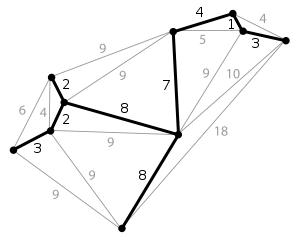
\includegraphics[width=110mm,height=70mm]{1.png}
\caption{ A planar graph and its minimum spanning tree. Each edge is labeled with its weight, which here is roughly proportional to its length.\label{overflow}}
\end{figure}

\section{Descrierea aplicatiei}
Pentru a reprezenta un graf, într-un program, am folosit structuri de date ce reprezinta graful prin  matricea sa de adiacenta. Problema se rezolva folosind algoritmul Greedy. Am creat functii pentru rezolvarea fiecarui algoritm.
Pentru realizarea grafului , am folosit structurile:
\begin{itemize}
  \item [i)]{\bf struct edge},cu ajutorul careia am definit 2 noduri u si v si muchia dintre respectivele noduri (w),care semnifica costul distantei.
  \item [ii)]{\bf struct edgelist} , in care am definit un vector ce retine lista muchiilor ( data[MAX]) si numarul lor (n).
\end{itemize}
In continuare,am definit urmatoarele functii ajutatoare  :
\begin{itemize}
  \item [i)]Functia\ {\bf sort()},ce ordoneaza crescator lista muchiilor in funcie de costul fiecareia.
  \item [ii)]Functia\ {\bf find()}, ce cauta in vectorul belongs[] valoarea careia ii apartine respectivul cost
  \item [iii)]Functia\ {\bf union1()}, ce uneste varfurile cu muchia data.
  \item [iiii)]Functia\ {\bf print()},afiseaza pe fiecare coloana varfurile si muchia dintre ele.In finalul functiei afisam costul minim. \end{itemize}  
Descrierea functiilor principale ale acestui proiect:
\begin{enumerate}
  \item [1.]Functia\ {\bf int prims ()} ce creaza matricele cost[][] si spanning[][].Initializam vectorii visited[],distance[] si from[],costul minim si numarul de muchii.Cautam varful aflat la distanta minima fata de arbore,apoi adaugam muchiile in arborele minim. 
  \item [2.]Functia\ {\bf void kruskal } . Parcurgem lista muchiilor astfel incat sa retinem fiecare 2 noduri si muchia dintre ele,respectiv costul acesteia. Apoi sortam cu ajutorul functiei sort() nodurile in functie de cost. Retinem costurile intr-un vector (belongs[]). Cream lista muchiilor ce urmeaza sa fie adaugate in minimum spanning tree.Conectam nodurile cu muchiile date. Conectand nodurile,in cazul in care se formeaza un ciclu,eliminam muchia respectiva.Repetam pasii pana ajungem la sfarsitul listei de muchii.
  
  
 
  \item [6.]Functia\ {\bf int main()},cuprinde declararea variabilelor: variabilele  total-cost ,iterator-rows, iterator-columns,aux  de tip int ;
  Citim din fisier matricea de adiacenta a grafului.
  Apelam functiile principale pentru rezolvarea problemei prin cei 2 algoritmi si afisam costul minim.

\end{enumerate}
\pagebreak

\section{Concluzii}
La prima vedere,sau mai bine spus,atunci cand citesti prima data cerinta problemei,nu pare deloc complicat,insa din punctul meu de vedere,cel mai greu a fost sa definesc functiile principale si cele ajutatoare ce rezolva problema prin 2 algoritmi.


\section{Bibliografie}

\begin{itemize}
  \item [i)] $The\ C\ Programming\ language,Second Edition$,Bian W. Kernighan,Dennis M. Ritchie
  \item [ii)] $\href{http://ad.becheru.net/}{Programming\ Techniques\ course}$
  \item [iii)] $\href{https://www.thecrazyprogrammer.com/}{The\ Crazy \ Programmer}$

\end{itemize}

\pagebreak



\end{document}
